\documentclass{article}

\usepackage{tikz}
\usetikzlibrary{mindmap,trees}
\usepackage{verbatim}

\begin{document}
\pagestyle{empty}

\hspace{-1 in} 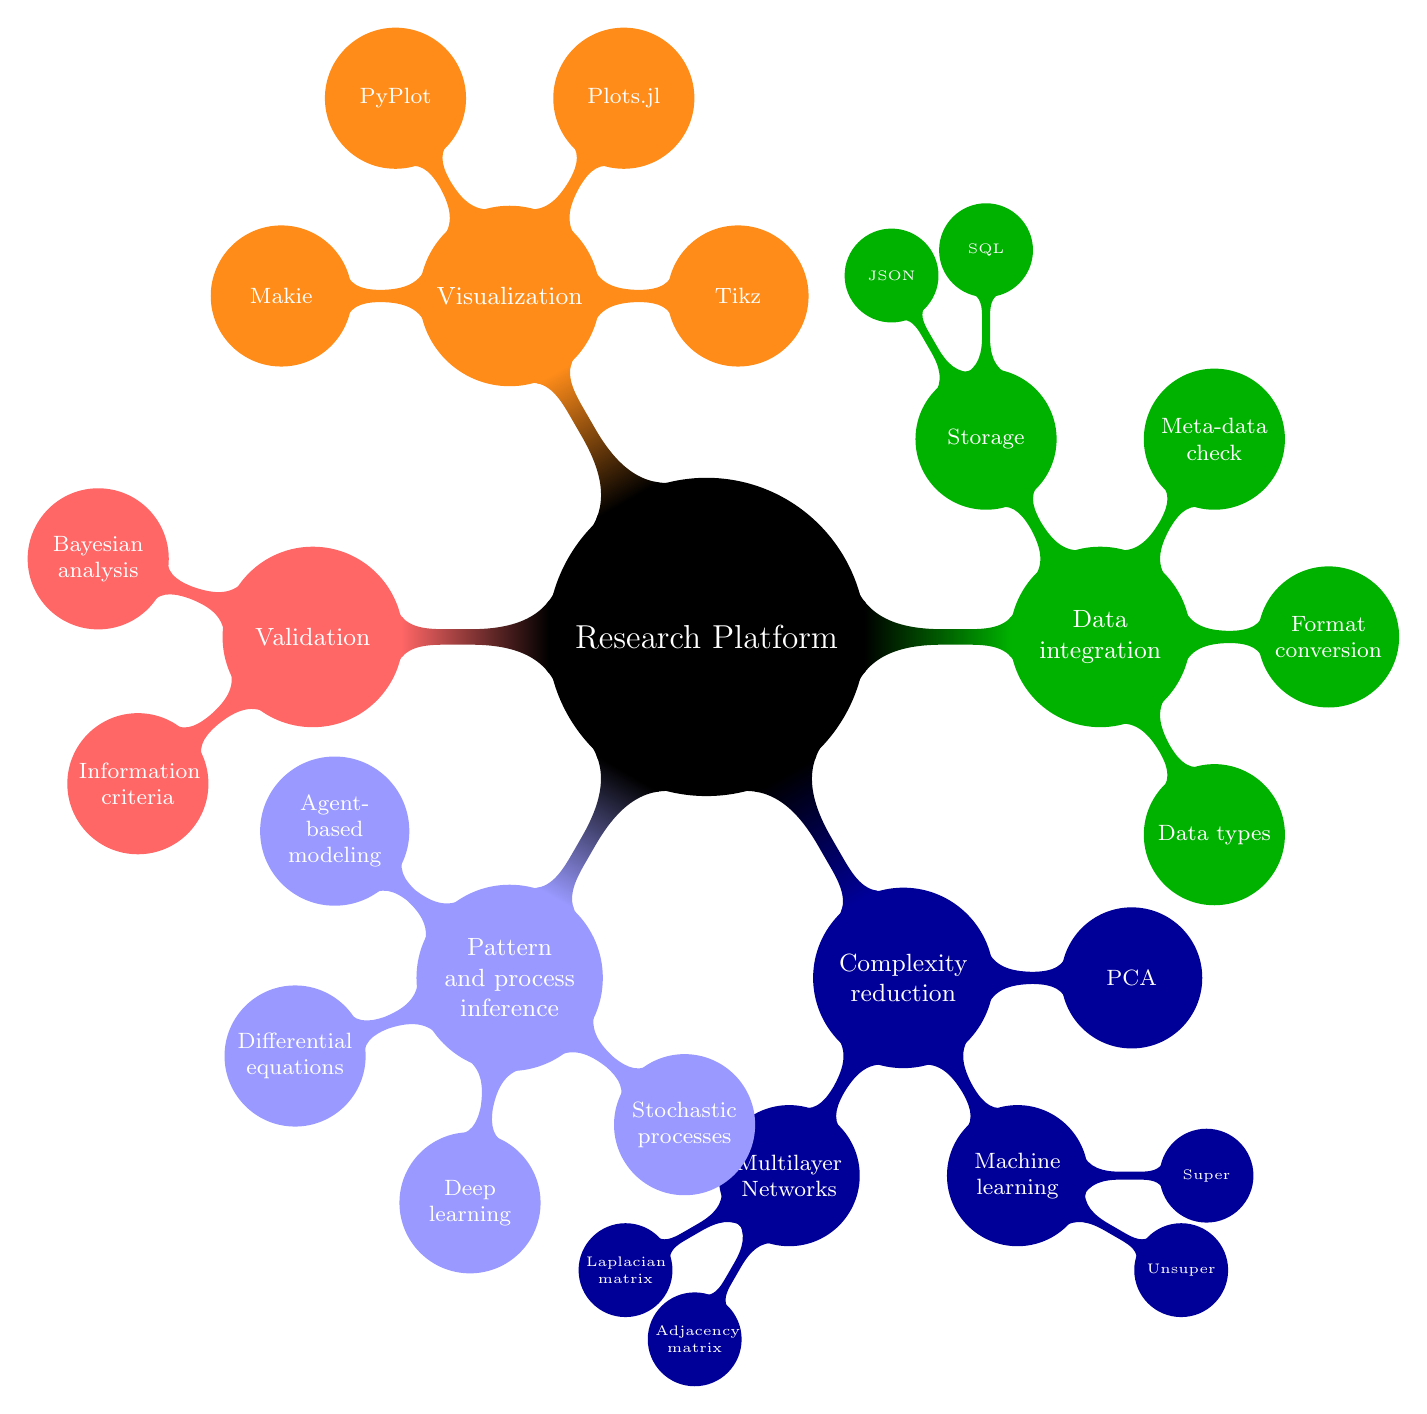
\begin{tikzpicture}
  \path[mindmap,concept color=black,text=white]
    node[concept] {Research Platform}
    [clockwise from=0]
    child[concept color=green!70!black] {
      node[concept] {Data integration}
      [clockwise from=120]
      child { node[concept] {Storage} 
      child {node[concept] {JSON}}
      child {node[concept] {SQL}}
      }
      child { node[concept] {Meta-data check} }
      child { node[concept] {Format conversion} }
      child { node[concept] {Data types} }
    }  
    child[concept color=blue!60!black] {
      node[concept] {Complexity reduction}
      [clockwise from=0]
      child { node[concept] {PCA} }
      child { node[concept] {Machine learning}
      child {node[concept] {Super}}
      child {node[concept] {Unsuper}}
      }
      child { node[concept] {Multilayer Networks}
        [clockwise from = 240]
      child {node[concept] {Adjacency matrix}}
      child {node[concept] {Laplacian matrix}}
      }
    }
    child[concept color=blue!40] {
      node[concept] {Pattern and process inference}
      [clockwise from=320]
      child { node[concept] {Stochastic processes} }
      child { node[concept] {Deep learning} }
      child { node[concept] {Differential equations} }
      child { node[concept] {Agent-based modeling} }
    }
    child[concept color=red!60] {
      node[concept] {Validation}
      [clockwise from=-140]
      child { node[concept] {Information criteria} }
      child { node[concept] {Bayesian analysis} }
    }
    child[concept color=orange!90] {
      node[concept] {Visualization}
      [clockwise from=180]
      child { node[concept] {Makie} }
      child { node[concept] {PyPlot} }
      child { node[concept] {Plots.jl} }
      child { node[concept] {Tikz} }
    }
    ;
\end{tikzpicture}
\end{document}